\chapter{Especificación de requerimientos}
\section{Pila de producto}
%Describa brevemente el producto en función del análisis de historias. Si es posible modifique la codificación de las historias para que el lector tenga un apoyo visual respecto a la estructura del sistema. Por ejemplo las historias correspondientes a los módulos de interfaz podrían codificarse UIXXX, mientras que las historias correspondientes a módulos de red podrían codificarse NTXXX. Explique en esta sección la lógica detrás de la codificación usada.

La pila de producto contiene las funcionalidades que se desean desarrollar para el sistema “Lector de PDF Minimalista”. Estas funcionalidades se expresan mediante historias de usuario, ya que permiten describir cada requerimiento desde la perspectiva de la persona que utilizará la aplicación.

Para identificar las historias se utiliza el código US, que significa User Story. La numeración se asigna de forma consecutiva. La columna Prioridad indica la importancia de cada funcionalidad para el proyecto, mientras que la columna Inserción señala si la historia formaba parte del alcance original o si fue agregada durante el Sprint 1. En el caso de que las tareas sean originales se encontrarán en color negro, si las tareas son nuevas se encontrarán en color verde y si fueron eliminadas se encontrarán en color rojo.

Las funcionalidades del producto se pueden dividir de la siguiente manera:
\begin{itemize}
    \item Interfaz minimalista y gestión general de la aplicación.
    \item Visualización, navegación y búsqueda dentro de documentos PDF.
    \item Edición, combinación y organización de páginas.
    \item Funcionalidades complementarias, como el modo presentación y la navegación mediante el outline.
    
\end{itemize}

\subsection{Requerimientos funcionales del sistema}

% La pila del producto debe actualizarla cada iteración del proyecto. Debe documentar los cambios sufridos durante la iteración pasada, de forma que se pueda trazar con mucho detalle los cambios que ha sufrido la definición del proyecto desde sus inicios. Si durante el desarrollo cambia alguno de los MVP o la EDT, debe modificarlos también y documentar la razón que justifica el cambio.

%% PILA DE PRODUCTO %%
\begin{longtable}{|l||p{7cm}|l|l|}

\multicolumn{4}{c}{Pila general del producto}\\
\hline\hline
\textbf{Código} & \textbf{Descripción} & \textbf{Prioridad} & \textbf{Inserción}\\
\hline
\endfirsthead
\textbf{Código} & \textbf{Descripción} & \textbf{Prioridad} & \textbf{Inserción}\\
\hline\hline
\endhead

%\textbf{RFXXX} & 
%\textbf{Título de la historia:} Descripción de la funcionalidad que representa la historia, lo más detallado posible y con énfasis en la implementación de funcionalidad. & Alta & Original\\

%\color{ForestGreen}
%\textbf{RF002} & Una historia nueva en este sprint & Media & Sprint 1 \\

%\color{Mahogany}
%\textbf{RF003} & Una historia eliminada & Baja & Original \\

\textbf{US-001} & 
\textbf{Aplicación de escritorio minimalista:} Como usuario, quiero una interfaz limpia y minimalista para la aplicación, de modo que pueda enfocarme en la lectura del contenido sin distracciones visuales. & Muy Alta & Original\\

\textbf{US-002} & 
\textbf{Compaginar archivos PDF:} Como usuario, quiero poder compaginar múltiples documentos o páginas, para organizar la estructura del documento final de manera lógica antes de exportarlo. & Media & Original\\

\color{Mahogany}
\textbf{US-003} & 
\textbf{Mezclar archivos PDF:} Como usuario, quiero poder intercalar o mezclar páginas de dos o más PDFs distintos, para consolidar información de múltiples fuentes en un solo archivo. & Alta & Original\\

\color{Mahogany}
\textbf{US-004} & 
\textbf{Abrir varios archivos PDF:} Como usuario, quiero tener la capacidad de abrir dos archivos PDF simultáneamente (en pantalla dividida o pestañas), para comparar su contenido o trabajar con ambos de forma paralela. & Media & Original\\

\textbf{US-005} & 
\textbf{Visualización ajustada al pdf:} Como usuario, quiero que la aplicación renderice y adapte correctamente la visualización del documento al tamaño de mi ventana con la función de prioridad en pantalla, para una experiencia ergonómica y de uso sobre otras aplicaciones. & Media & Original\\

\textbf{US-006} & 
\textbf{Presentar PDF:} Como usuario, quiero activar un modo de presentación a pantalla completa, para poder exponer el contenido del documento a una audiencia ocultando los menús y herramientas. & Media & Original\\

\textbf{US-007} & 
\textbf{Eliminar páginas de un PDF:} Como usuario, quiero poder seleccionar y eliminar páginas específicas de un PDF, para remover información irrelevante o incorrecta del documento original. & Media & Original\\

\textbf{US-008} & 
\textbf{Guardar un PDF:} Como usuario, quiero poder guardar los cambios realizados sobre el archivo PDF actual, para asegurar y no perder el progreso de mi edición. & Media & Original\\

\textbf{US-009} & 
\textbf{Reordenar páginas de un PDF:} Como usuario, quiero poder reordenar las páginas del documento (por ejemplo, arrastrándolas), para ajustar el flujo de lectura y la organización según mis necesidades. & Media & Original\\

\textbf{US-010} & 
\textbf{Outline del PDF:} Como usuario, quiero visualizar el índice (outline) del documento en un panel lateral, para comprender rápidamente la jerarquía y estructura general del texto. & Media & Original\\

\textbf{US-011} & 
\textbf{Navegar Outline:} Como usuario, quiero poder hacer clic en cualquier sección del índice (outline) y saltar directamente a esa página, para navegar ágilmente a través de documentos muy extensos. & Media & Original\\

\textbf{US-012} & 
\textbf{Guardar nuevo PDF:} Como usuario, quiero tener la opción de "Guardar como" para generar un nuevo archivo con mis modificaciones, manteniendo el PDF original intacto como respaldo. & Media & Original\\

\textbf{US-013} & 
\textbf{Buscar Texto:} Como usuario, quiero utilizar una barra de búsqueda para encontrar palabras o frases específicas dentro del documento, para localizar datos puntuales sin tener que leer todo el texto. & Media & Original\\

\textbf{US-014} & 
\textbf{Abrir un PDF:} Como usuario, quiero poder abrir un archivo PDF desde el explorador de archivos de mi dispositivo, para acceder a su contenido dentro de la aplicación. & Muy Alta & Original\\

\textbf{US-015} & 
\textbf{Ver páginas de un PDF:} Como usuario, quiero poder visualizar las páginas individuales del documento, para poder consumir la información que contienen. & Media & Original\\

\textbf{US-016} & 
\textbf{Copiar texto portapapeles:} Como usuario, quiero poder copiar el texto previamente seleccionado al portapapeles del sistema, para pegarlo y reutilizarlo en otras herramientas o correos. & Media & Original\\

\textbf{US-017} & 
\textbf{Zoom de un PDF} Como usuario, quiero poder acercar (zoom in) y alejar (zoom out) la vista de la página, para visualizar detalles pequeños o evaluar la distribución completa de la hoja. & Media & Original\\

\textbf{US-018} & 
\textbf{Scroll de un PDF:} Como usuario, quiero poder desplazarme verticalmente (scroll) a lo largo del documento, para mantener una experiencia de lectura continua y fluida. & Media & Original\\

\textbf{US-019} & 
\textbf{Seleccionar texto:} Como usuario, quiero poder seleccionar bloques de texto arrastrando el cursor, como acción indispensable antes de poder copiar o resaltar el contenido. & Media & Original\\

\textbf{US-020} & 
\textbf{Saltar a Página:} Como usuario, quiero poder ingresar un número específico de página, para saltar a esta inmediatamente sin tener que scrollear & Media & Original\\

\textbf{US-021} & 
\textbf{Mostrar Conteo de Páginas:} Como usuario, quiero poder la página en la que estoy en relación a la cantidad total de páginas, para saber con certeza en que parte del documento me encuentro. & Media & Original\\

\textbf{US-022} & 
\textbf{Menú Click Derecho:} Como usuario, quiero poder mostrar un menú con click derecho, para acceder a todas las funcionalidades del sistema sin que estas se entrometan en el lector. & Media & Original\\
\hline

%Sprint 2

\textbf{US-023} & 
\textbf{Firmar el documento abierto con GAUDI:} Como persona usuaria con tarjeta de firma digital quiero firmar el PDF que tengo abierto sin salir de la aplicación para no tener que abrir otro programa para firmarlo. & Alta & Original\\
\hline

\textbf{US-024} & 
\textbf{Ver el estado de firma del documento:} Como usuario que recibe un PDF
quiero saber si el documento está firmado digitalmente y por quién
para confiar de su procedencia. & Alta & Original\\
\hline

\textbf{US-025} & 
\textbf{Resaltar texto seleccionado:} Como usuario que estudia un documento quiero resaltar fragmentos de texto para poder verlos claramente y diferenciarlos entre el texto. & Media & Original\\
\hline

\textbf{US-026} & 
\textbf{Elegir el color del resaltado:} Como persona usuaria quiero escoger entre varios colores de resaltado para clasificar lo que marco. & Baja & Original\\
\hline

\textbf{US-027} & 
\textbf{Eliminar un resaltado:} Como persona usuaria quiero quitar un resaltado que ya no necesito para mantener el documento limpio. & Media & Original\\
\hline

\textbf{US-028} & 
\textbf{Guardar los resaltados en el archivo:} Como usuario quiero que los resaltados que hice se guarden cuando guardo el archivo para encontrarlos la próxima vez que lea el documento. & Media & Original\\
\hline

\textbf{US-029} & 
\textbf{Agregar un comentario a una selección:} Como usuario quiero agregar un comentario de texto a cualquier parte del documento que haya seleccionado, para poder hacer anotaciones sobre el documento en el mismo archivo y no tener que crear otro. & Media & Original\\
\hline

\textbf{US-030} & 
\textbf{Leer, editar y eliminar comentarios:} Como usuario quiero leer los comentarios que vengan en un documento, así como editarlos o eliminarlos, para poder leer los comentarios de otras personas y para modificarlos antes de enviar el documento a alguien más. & Alta & Original\\
\hline

\textbf{US-031} & 
\textbf{Listar los comentarios en el panel lateral:} Como persona que revisa un documento largo quiero ver todos los comentarios en una lista para recorrerlos sin buscarlos página por página & Media & Original\\
\hline

\textbf{US-032} & 
\textbf{Guardar los comentarios en el archivo:} Como usuario quiero que los resaltados que hice se guarden cuando guardo el archivo para encontrarlos la próxima vez que yo, o alguien más, lea el documento. & Alta & Original\\
\hline

\textbf{US-033} & 
\textbf{Insertar una imagen de firma en el documento:} Como persona usuaria quiero colocar la imagen de mi firma en una página para dejar constancia visual en el documento de que se firmó. & Media & Original\\
\hline

\textbf{US-034} & 
\textbf{Mover y redimensionar la firma antes de fijarla:} Como persona usuaria quiero ajustar dónde y de qué tamaño queda mi firma para que caiga sobre la línea correcta del documento. & Media & Original\\
\hline

\textbf{US-035} & 
\textbf{Guardar la imagen de firma para reutilizarla:} Como persona que firma documentos seguido quiero guardar mi imagen de firma en la aplicación para no buscar el archivo cada vez. & Baja & Original\\
\hline

\textbf{US-036} & 
\textbf{Distinguir la firma gráfica de la firma digital:} Como persona usuaria quiero entender que la imagen no da validez legal al documento para no confiarme de una firma que no está verificada. & Media & Original\\
\hline

\textbf{US-037} & 
\textbf{Instalador que configura extensiones en windows:} Como usuario quiero poder instalar la aplicación en mi sistema para que se configure dentro del sistema operativo y sea más fácil utilizarla por medio del menú de inicio, en el escritorio, o simplemente abriendo un documento. & Media & Original\\
\hline

\textbf{US-038} & 
\textbf{Usar 'Abrir con' de windows para abrir la app:} Como usuario quiero que cuando selecciono un pdf en windows y uso la función de “abrir con”, la aplicación debería desplegarse con el pdf cargado para que me sea más fácil abrir cualquier documento. & Media & Original\\
\hline

\textbf{US-039} & 
\textbf{Mostrar anotaciones:} Como usuario, quiero poder ver las anotaciones que tiene un documento que fueron hechas con otro editor, para poder visualizar toda la información del documento. & Media & Original\\
\hline


\caption{\color{ForestGreen}VERDE: Historias agregadas en esta iteración. \color{Mahogany}ROJO: Historias eliminadas.}
\label{ProductBacklog}

\end{longtable}

\subsection{Bitácora de cambios}
%Documente en esta sección las decisiones que llevaron a la creación de nuevas historias, o la eliminación de historias ya analizadas. Detalle con cuidado todas las historias afectadas con su respectivo código, indicando por qué razón fue eliminada / agregadas a la pila.

\subsubsection{Iteración 1}

Durante el desarrollo del sprint fue necesario agregar algunas correcciones denotadas con el código FX-\#\#\#\#.
\begin{itemize}
    \item FX-001: Presentar toma URL en vez de PDF.
    \item FX-002: Unir Viewer y PresentationViewer con OpenFile.
    \item FX-003: Unir Zoom con Viewer
    \item FX-004: Refactorizar código para que esté en línea con el estándar.
\end{itemize}

Se decidió eliminar las historias de usuario US-003: Mezclar archivos PDF y US-004: Abrir varios archivos PDF. Esto debido a que son funcionalidades complejas que toma mucho tiempo implementar, además durante el desarrollo se descubrió que está funcionalidad se podía replicar usando las funciones de compaginar y reordenar.

\subsubsection{Iteración 2}


\section{Producto Mínimo Viable de la iteración 2}
%Amplíe en esta sección la descripción del MVP que corresponde a la iteración en curso, indique con mayor detalle qué funcionalidades engloba.

El producto mínimo viable de está iteración es una extensión de las funcionalidades del lector y editor de documentos PDF desarrollado en la etapa anterior. Las nuevas funcionalidades comprenden los comentarios, highlights, firma digital e instalación del programa.

El producto es capaz de firmar documentos de forma digital siguiendo la reglamentación que impone el Banco Central de Costa Rica. Además, la firma se puede incluir de forma gráfica, siempre advirtiendo al usuario sobre la diferencia de validez de una firma solamente gráfica y una digital.

También, se pueden agregar, eliminar, modificar y leer comentarios y highlights que están en el documento. Por lo tanto, la función de guardar se extiende para incluir estás anotaciones.

Está iteración del producto mejora su instalación dentro del sistema operativo del usuario ofreciendo opciones para asociar el programa con los documentos PDF, asi como crear íconos en el escritorio.

\subsection{Pila de trabajo de la iteración 2}

%Describa la capacidad instalada de su equipo de trabajo, incorpore información que describa, para esta iteración, cuál es el presupuesto disponible en puntos de historia. Indique también si algún miembro del equipo tiene un rol especializado y cuántas horas le dedicará al rol respectivo.

El presupuesto disponible en puntos de historia es de 72 puntos como se muestra en el cuadro 2.2. La carga total fue de 63 puntos que ronda aproximadamente el 87.5\% de capacidad. El planeamiento inicial se planteó con el fin de dejar espacio para resolver posibles problemas, sobrellevar alguna mala estimación de puntos por tarea y agregar funcionalidades extra (si se determinan necesarias) que complementen la aplicación. 

\begin{longtable}{|l|l|l|}
    \hline
    \textbf{Miembro del equipo} & \textbf{Rol} & \textbf{Capacidad} \\
    \hline
    Fabián Araya & Desarrollador y SCRUM Master & 12 \\
    Samuel Zúñiga & Desarrollador & 12 \\
    Rubén Hurtado & Desarrollador & 12\\
    Andrés Feng & Desarrollador & 12\\
    Xotchil Rojas & Desarrollador & 12\\
    Víctor Mejías & Desarrollador & 12 \\
    \hline \hline
    \textbf{Presupuesto total:} &  & 72\\
    \hline
    \caption{Resumen de capacidad de carga del equipo para la iteración 2}
\end{longtable}


En la planeación del sprint y durante el desarrollo se agregan tareas que no se clasifican como historias de usuario y solo son relevantes para esta iteración específica. Estas tareas se clasifican en tres tipos: Task(código TK), Documentación (código DC) y Fix (código FX); y se les asigna un consecutivo al igual que las historias de usuario.

En este sprint se asignaron las siguientes tareas:
\begin{itemize}
    \item TK-002: Investigar como implementar GAUDI
    \item FX-005: Comunicación de Presentation a Viewer
    \item FX-006: Corregir posición y estilo de conteo de páginas - estilo de la barra de desplazamiento
    \item FX-007: Refactor de delete pages para que esté en el outline
    \item FX-008: Mejoras de UX en función Reordenar Páginas
    \item FX-009: Arreglar sombras del visualizador
    \item FX-010: Comentarios en páginas agrupados
    \item DC-001: Manual de Usuario
    \item DC-002: Manual Técnico
    \item DC-003: Informe de Avance Incompleto
    \item DC-004: Informe de Avance Completo
\end{itemize}


%% PILA DEL SPRINT (ITERACIÓN) %%

\begin{longtable}{|l||c|c|p{7cm}|l|}

\multicolumn{5}{c}{Pila de la \textbf{iteración 2} }\\
\hline\hline
\textbf{Código} & \textbf{CE} & \textbf{CR} & \textbf{Responsables} & \textbf{Finalización} \\
\hline
\endfirsthead
\textbf{Código} & \textbf{CE} & \textbf{CR} & \textbf{Responsables} & \textbf{Finalización} \\
\hline\hline
\endhead

\textbf{US-023} & 4 &  & Responsable A, Responsable B & 2017/08/14 \\
\textbf{US-024} & 2 &  &  &  \\
\textbf{US-025} & 2 &  &  &  \\
\textbf{US-026} & 3 &  &  &  \\
\textbf{US-027} & 3 &  &  &  \\
\textbf{US-028} & 3 &  &  &  \\
\textbf{US-029} & 3 &  &  &  \\
\textbf{US-030} & 4 &  &  &  \\
\textbf{US-031} & 3 &  &  &  \\
\textbf{US-032} & 2 &  &  &  \\
\textbf{US-033} & 4 &  &  &  \\
\textbf{US-034} & 2 &  &  &  \\
\textbf{US-035} & 1 &  &  &  \\
\textbf{US-036} & 2 &  &  &  \\
\textbf{US-037} & 2 &  &  &  \\
\textbf{US-038} & 2 &  &  &  \\
\textbf{US-039} & 1 &  &  &  \\
\textbf{TK-002} & 4 &  &  &  \\
\textbf{FX-005} & 1 &  &  &  \\
\textbf{FX-006} & 1 &  &  &  \\
\textbf{FX-007} & 1 &  &  &  \\
\textbf{FX-008} & 2 &  &  &  \\
\textbf{FX-009} & 1 &  &  &  \\
\color{ForestGreen}
\textbf{FX-010} & 1 &  &  &  \\
\textbf{DC-001} & 2 &  &  &  \\
\textbf{DC-002} & 3 &  &  &  \\
\textbf{DC-003} & 2 &  &  &  \\
\textbf{DC-004} & 2 &  &  &  \\


\hline
Total & 10 & 12 & & \\
\hline

\caption{Pila de la Iteración 2. \textbf{CE:} Carga Estimada, \textbf{CR:} Carga Real.}
\label{SprintBacklog}

\end{longtable}

\subsection{Desempeño del equipo}
%Documente cualquier problema que se haya presentado durante el desarrollo. Describa las situaciones que se presentaron por las cuales fue necesario cambiar la pila de trabajo planificada (si hubieran).

%Incluya la gráfica de quemado e incorpore la siguiente información: Velocidad del equipo, carga estimada total, carga real total.

% Gráfica de quemado
\begin{figure}[H]
  \centering
    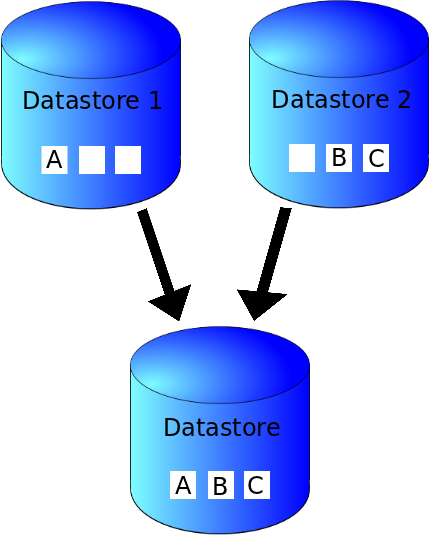
\includegraphics[height= 10cm, width=15cm]{project/images/data-sync}
  \caption{\textbf{IMAGE CAPTION}}
\end{figure}

%Si la carga estimada y la carga real difieren, explique porqué se da la diferencia.